\begin{corollary}
  If a graph \(G = (V, E)\) satisfies \(|E| > 3|V| - 6\), then 
  the graph is non-planar. 
\end{corollary}

\begin{nexample}
  Consider the graph \(K_5\). Notice that
  \[ m = \binom{5}{2} = 10 > 3\cdot5 - 6 = 9 \]
  Thus, \(K_5\) is not planar. Similarly, since \(K_5 \subseteq
  K_6\), \(K_6\) is also non-planar.
\end{nexample}

\begin{remark}
  If a non-planar graph \(H\) is a subgraph of \(G\), then \(G\)
  is non-planar as well.
\end{remark}

\begin{remark}
  It is possible to find a non-planar graph with \(m \leq 3n-6\).
\end{remark}

\begin{theorem}
  \(K_{3, 3}\) is non-planar.
\end{theorem}

\begin{proof}
  Notice that in a bipartite graph, every face must be adjacent
  to \(\geq 4\) edges since a face is made of cycles and each 
  cycle must be even in bipartite graphs. Then, we would have
  that
  \begin{equation}
    4F \leq M \leq 2E \implies 2F \leq E
    \label{eq:k33-non-planar}
  \end{equation}

  Suppose to contradict that \(K_{3, 3}\) is planar. Then,
  \[
    \begin{aligned}
      V - E + F &= 2 \\
      F &= 2 + E - V \\
    \end{aligned}
  \]
  Combining with Equation \ref{eq:k33-non-planar}, we would have
  \[
    \begin{aligned}
      \frac{E}{2} &\geq 2 + E - V \\
      E &\geq 4 + 2E - 2V \\
      2V - 4 &\geq E \\
      2 \cdot 6 - 4 &\geq 9 \\
      8 &\geq 9
    \end{aligned}
  \]
  This is a contradiction. Therefore, \(K_{3, 3}\) cannot be
  planar.
\end{proof}

\begin{theorem}
  A graph \(G\) of order \(n \geq 3\) and size \(m\) is
  non-planar if any of the following occurs:
  \begin{enumerate}[label=(\arabic*.)]
    \item \(m > 3n-6\); or
    \item \(G\) contains \(K_5\) as a subgraph; or
    \item \(G\) contains \(K_{3, 3}\) as a subgraph.
  \end{enumerate}
\end{theorem}

\begin{remark}
  There is a non-planar graph \(G\) that \(m \leq 3n - 6\) and
  \(G\) does not contain \(K_5\) or \(K_{3, 3}\) as a subgraph.
\end{remark}

\section{Subdivision}

\begin{definition}[Subdivision]
  A graph \(G'\) is called a \textit{subdivision} of a graph
  \(G\) if \(G' = G\) or one or more vertices of degree 2 are
  inserted into one or more edges of \(G\).
\end{definition}

\begin{figure}[ht]
\begin{nexample}
  Below, we can see that all of \(G, G_1, G_2, G_3\) are
  subdivisions of \(G\). Note that \(G_2\) is a subdivision of
  \(G_1\) as well.

  \centering
  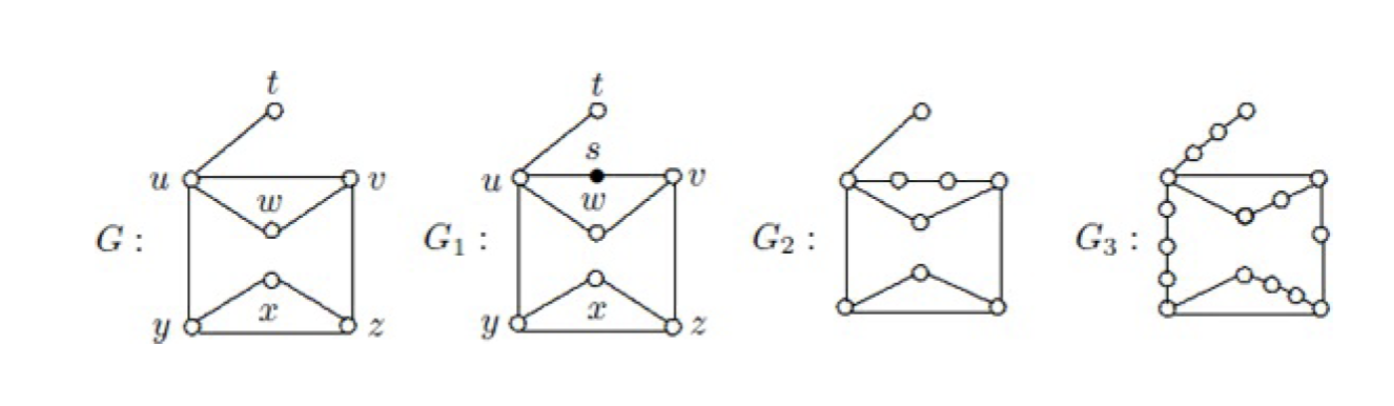
\includegraphics[width=0.95\textwidth]{figures/l13/subdiv-example}
\end{nexample}
\end{figure}

\begin{theorem}[Kuratowski's Theorem, 1930]
  A graph \(G\) is planar if and only if \(G\) does not contain a
  subdivision of \(K_5\) or \(K_{3, 3}\) as a subgraph.
\end{theorem}

\begin{figure}[ht]
\begin{nexample}
  We claim that the graph below is non-planar. We can see that we
  construct a subdivision of \(K_{3, 3}\) graph with \(A = \{v_1,
  u_2, y_1\}\) and \(B = \{v_2, u_1, y_2\}\).

  Then, by Kuratowski's Theorem, we have that this graph is
  non-planar.
\end{nexample}
\end{figure}

\section{Graph Minors}

\begin{definition}[Edge Contraction]
  For a graph \(G\) and an edge \(e=u v\) of \(G\), a graph 
  \(G^{\prime}\) is said to be obtained from \(G\) by
  \textit{contracting the edge} \(e\) if \(G^{\prime}\) is
  (isomorphic to) the graph
  obtained by joining \(u\) in the graph \(G-v\) to any neighbor
  of \(v\) not already adjacent to \(u\).
\end{definition}

\begin{definition}[Graph Minors]
  A graph \(H\) is called a \textit{minor} of a graph \(G\) if
  (a graph isomorphic to) \(H\) can be obtained from \(G\) by a
  succession of edge contractions, edge deletions, or vertex
  deletions (in any order). 
\end{definition}

\begin{theorem}
  If a graph \(G\) is a subdivision of a graph \(H\), then \(H\)
  is a minor of \(G\).
\end{theorem}

Notice that being a graph minor is a stronger condition than a
subdivision.

\begin{theorem}[Wagner's Theorem, 1937]
  A graph \(G\) is planar if and only if neither \(K_5\) nor
  \(K_{3, 3}\) is a minor of \(G\).
\end{theorem}

